\documentclass[acmsmall,screen,review,anonymous]{acmart}

\usepackage{amsmath}
\usepackage{tabularx}
\usepackage{tikz}
\usetikzlibrary{arrows.meta,positioning}

\setcopyright{none}
\acmConference[FSE 2027]{ACM International Conference on the Foundations of Software Engineering}{12--16 July 2027}{Shenzhen, China}
\acmBooktitle{ACM International Conference on the Foundations of Software Engineering (FSE 2027), 12--16 July 2027, Shenzhen, China}
\acmYear{2027}
\copyrightyear{2027}
\acmDOI{}
\acmISBN{}

\title[Role Labels and Call Topology]{Role Labels or Extra Calls? A Controlled Study of Quality and Cost in LLM Code Generation}

\begin{abstract}
LLM code-generation workflows often combine named roles with multiple model calls, obscuring which choice changes quality and resource use. We separate these choices in a crossed experiment: neutral versus planner--implementer--reviewer labels, and one versus three calls, with identical operations and full task context; a direct solver is a fifth condition. GPT-5.6 Luna received 15,000 assignments on 1,000 BigCodeBench tasks, with three fresh requests per task and condition. Generation completed for 14,961 assignments, and 985 tasks met the control-gate criteria. Role labels change paired success by $-0.75$ percentage points in one call and $+1.35$ points in three calls; neither null hypothesis is rejected after Holm correction. This does not establish equivalence. Three calls reduce paired success by 4.17 points under neutral labels and 2.13 points under role labels. On complete resource pairs, API-equivalent valuation increases by factors of 2.67 and 2.78. The negative call-structure result persists under a source-dependence audit specified during generation and in 800 newly sampled task IDs. An earlier GPT-5.4-mini study on the same 200 task IDs yields the same directions for all four contrasts, although none of its four tests rejects after correction. In a separate 2,000-block comparison, adapted Self-Collaboration has lower success on observed task pairs and approximately three times the valuation, but infrastructure-related missingness prevents a full-population quality ranking. For the tested full-context function-generation workflows, role labels show no reliable benefit, while three calls lower executable success on complete eligible quality pairs and increase valuation on complete resource pairs.
\end{abstract}

\ccsdesc[500]{Software and its engineering~Automatic programming}
\ccsdesc[300]{Software and its engineering~Software testing and debugging}
\keywords{LLM code generation, orchestrated prompting, role prompting, factorial experiment, executable evaluation, resource accounting}

\begin{document}
\maketitle
\section{Introduction}
Code-generation workflows increasingly assign planning, implementation, and review to named LLM roles. Systems such as Self-Collaboration, ChatDev, MetaGPT, AgentCoder, and PairCoder combine role specialization with interaction, generated tests, tool use, or repeated refinement~\cite{dong2023selfcollaboration,qian2024chatdev,hong2024metagpt,huang2023agentcoder,zhang2024paircoder}. End-to-end comparisons cannot isolate whether reported gains arise from the role names, the operations, additional calls, feedback, or extra computation. That distinction matters in software engineering: each added call can retransmit a large repository context, expose an unverified intermediate response, and increase cost. The primary experiment evaluates sequential prompts sent to one model. Multi-agent systems motivate the design, but the experiment does not test independent agents.

We study a deliberately narrow workflow. The model is asked to analyze requirements and edge cases, implement a solution based on that analysis, and review and revise the program. Correctness is then measured by executing the original benchmark tests in a pinned offline environment; the model's textual assertion is never an outcome. We cross two factors while keeping operation sentences and supplied context fixed: neutral versus role labels, and one versus three fresh calls. A direct one-call solver serves as the simpler baseline.

The study asks three research questions. \textbf{RQ1:} Do role labels change executable success when the requested operations and call structure are held fixed? \textbf{RQ2:} Does splitting those operations across three full-context calls change success and measured resources relative to one call? \textbf{RQ3:} How do the staged workflows compare with a direct solver and with a published analyst--developer--tester controller? The first two questions form the prespecified factorial analysis. Comparisons with the direct baseline, the role-by-topology interaction, and subgroup checks are labeled exploratory. The external-controller study has its own prespecified hypothesis-testing family and missingness analysis.

The labels \texttt{planner}, \texttt{implementer}, and \texttt{reviewer} denote prompt segments; they do not imply distinct underlying agents, separate memories, or separate optimization processes. The experiment uses 1,000 BigCodeBench tasks with three fresh requests per condition, and the analysis includes all 14,961 completed candidates. The expanded sample contains 200 task IDs from the earlier study and 800 newly sampled IDs; all responses were regenerated. We report the 200/800 sensitivity separately and do not call the full sample an independent 1,000-task replication.

We use a crossed design to separate lexical role labels from call topology and report task-paired quality and resource estimates with missingness bounds and a source-dependence audit specified during generation. We then compare the primary results with GPT-5.4-mini, a direct solver, and an adapted Self-Collaboration controller. The direct and interaction comparisons are exploratory, and the study does not claim a general multi-agent effect. In this full-context setting, role labels do not yield a reliable quality benefit, while three-call execution costs substantially more and succeeds less often than the matched one-call workflow.

\section{Related Work and Scope}
Self-Collaboration decomposes code generation into analyst, developer, and tester roles, reports role and interaction-count ablations, and measures token cost~\cite{dong2023selfcollaboration}. ChatDev and MetaGPT coordinate specialized roles across broader software-development processes~\cite{qian2024chatdev,hong2024metagpt}. AgentCoder closes a generated-test feedback loop among programmer, test designer, and executor; PairCoder at ASE couples navigator and driver roles with multi-plan exploration and execution feedback~\cite{huang2023agentcoder,zhang2024paircoder}. MapCoder combines retrieval, planning, coding, and debugging roles~\cite{islam2024mapcoder}. AdaCoder evaluates four frameworks across 12 open-source models before adding adaptive planning and feedback~\cite{zhu2026adacoder}; a distinct ACL paper also named PairCoder evaluates a lighter two-agent scheme across 13 models and explicitly measures tokens~\cite{chen2026paircoder}. A systematic review identifies 71 primary studies of LLM multi-agent systems for software engineering and highlights the unresolved need to isolate agent capabilities from collaboration effects~\cite{he2025lma}.

Recent controlled comparisons examine homogeneous workflows reproduced by one model, adaptive topology selection, and quality--cost trade-offs~\cite{xu2026oneflow,hong2026dats,kapoor2025agents}. These studies vary complete architectures, allocate different compute, or use executable feedback. We instead vary lexical role labels and call boundaries while holding operation sentences and supplied context fixed. Self-Collaboration is the closest prior workflow. It already compares role-playing instructions with a zero-shot version that removes role-playing and slightly rewrites the operation sentences for naturalness. Our study holds those sentences unchanged and crosses lexical labels with one versus three calls, using repeated task-paired outcomes, full-context resource accounting, and explicit treatment of missing outcomes. Our separate SCC comparison adapts its analyst--developer--tester controller to the same model, tasks, and external evaluator and documents the changes required for this setting. INoT motivates compact internal dialogue and role-like reasoning instructions~\cite{sun2025inot}; we exclude it from the primary factorial family because it changes the reasoning procedure.

\begin{table}[t]
\caption{Closest code-generation workflow studies. Execution feedback means runtime test or trace outcomes returned during generation. Resource reporting includes token or call accounting. SCC feedback varies by configuration: its published compiler variant and our adapted author controller execute checks. SCC also studies role removal; our factorial intervention keeps operation sentences unchanged.}
\label{tab:related-designs}
\centering\scriptsize
\begin{tabularx}{\linewidth}{@{}lXccc@{}}
\toprule
Work & Primary variation & Execution feedback & Resources & Direct baseline\\
\midrule
SCC~\cite{dong2023selfcollaboration} & Role configurations and turns & Varies & Yes & Yes\\
MapCoder~\cite{islam2024mapcoder} & Four-role repair pipeline & Yes & Yes & Yes\\
AdaCoder~\cite{zhu2026adacoder} & Adaptive planning across models & Yes & Yes & Yes\\
PairCoder~\cite{chen2026paircoder} & Two-agent switching across models & No & Yes & Yes\\
OneFlow~\cite{xu2026oneflow} & Multi- versus single-model execution & Varies & Yes & Yes\\
DATS~\cite{hong2026dats} & Five task-adaptive topologies & Varies & Yes & Yes\\
This work & Labels $\times$ one/three calls & No & Yes & Yes\\
\bottomrule
\end{tabularx}
\end{table}


Persona prompting studies likewise distinguish a named persona from a demonstrated performance benefit~\cite{zheng2024personas,araujo2025personas}. Self-Refine and Reflexion use feedback and revision~\cite{madaan2023selfrefine,shinn2023reflexion}. Execution-guided methods such as CodeT and LDB use generated tests or runtime traces to select or repair programs~\cite{chen2023codet,zhong2024ldb}. Feedback and revision can improve code generation. Execution-guided variants also bundle workflow structure with executable feedback. Our primary matrix withholds all executable feedback until generation ends, so it estimates the effects of labels and call boundaries rather than those of execution-guided repair.

Comparisons involving additional calls can confound call count with computation, repeated context, and exposure of intermediate responses. Matched-thinking-budget work emphasizes that these are distinct interventions~\cite{tran2026budget}. Cost-aware agent evaluation likewise argues for joint accuracy--cost reporting and strong simple baselines~\cite{kapoor2025agents}. Our topology contrast includes repeated context, additional generation, and exposure of intermediate responses. We report each resource component and did not impose a post hoc output budget. Agentless and SWE-agent add localization, repository access, or tool interaction~\cite{xia2025agentless,yang2024sweagent}; those systems address a broader repository setting than the fixed-context function-generation setting studied here. BigCodeBench supplies diverse library-dependent tasks with executable tests~\cite{zhuo2024bigcodebench}. Native evaluation improves auditability while remaining subject to the benchmark's task--test limitations.

\section{Workflow and Estimands}
An engineering task is $(x,\mathcal{C}_0,\mathcal{V})$, where $x$ is the specification, $\mathcal{C}_0$ is the complete supplied context, and $\mathcal{V}$ is an external verification procedure. A protocol $a$ produces a candidate program $y$ and a verification record. In the primary study, $r=1,2,3$ indexes the three requests for task $t$. When its outcome is available, $Y_{tr}(a)\in\{0,1\}$ records whether the candidate passes the original tests in a valid environment. Missing outcomes remain undefined. For tasks with all three outcomes, $\bar Y_t(a)=\frac{1}{3}\sum_{r=1}^{3}Y_{tr}(a)$ is the per-generation success mean. Each primary contrast averages differences between these means over eligible tasks with all six required outcomes. Thus its estimand is conditional on a complete pair, with equal task weights. We report quality and resources separately because no externally justified joint utility or quality-loss margin is available.

In the single-call core, one model call receives $x$, $\mathcal{C}_0$, and three ordered operations: analyze requirements and edge cases; implement using the plan; review and revise against the requirements. It returns exactly one fenced Python program. The hidden reasoning trace is unavailable and is not treated as an observed plan or critique score. In the multi-call version, the same three operations are assigned to three fresh calls. Call $j$ receives the task, unchanged context, and every complete preceding response. The final response supplies the candidate. No benchmark test, reference solution, or evaluator feedback is returned to the model.

The five conditions are D (direct implementation), SN (neutral stage labels in one call), SR (role labels in one call), MN (neutral labels across three calls), and MR (role labels across three calls). All structured conditions use identical operation sentences and final-output contract. The label intervention replaces stage names with \texttt{planner}, \texttt{implementer}, and \texttt{reviewer}. The topology contrast includes repeated full-context transmission and intermediate-response exposure; it is not an effect of call count alone.

The observable state after call $j$ is $\sigma_j=(x,\mathcal{C}_0,a,j,\mathcal{H}_j)$, where $\mathcal{H}_j$ contains complete preceding responses. Generation runs sequentially until the assigned number of calls is complete, or a call is incomplete. Resource availability is checked separately from candidate quality. Incomplete assignments remain unavailable and are not retried automatically. A completed response with zero or multiple recognized Python fences yields an empty observed candidate and a format-error flag. The evaluator then records pass, failure, or unavailable. Only external test execution determines $Y_{tr}(a)$.

Let $L$ be the token length of the task and context, $H_j$ the instruction overhead, $E_j$ the exposed answer length, and $O_j$ all output tokens of call $j$. Hidden reasoning may contribute to $O_j$ but is not forwarded in $E_j$. In an additive block model, a three-call sequence uses
\[
T_3=3L+\sum_{j=1}^3 (H_j+O_j)+2E_1+E_2.
\]
A single call uses $T_1=L+H_s+O_s$. Thus repeated context contributes $2L$ to the difference, while overhead, exposed history, and output lengths account for the remaining terms. The net token difference, $T_3-T_1$, need not be positive. Because tokenizer boundaries are nonadditive, reported resource values use provider counters. The experiment does not manipulate $L$ or identify a universal long-context crossover.

\begin{figure*}[t]
\centering
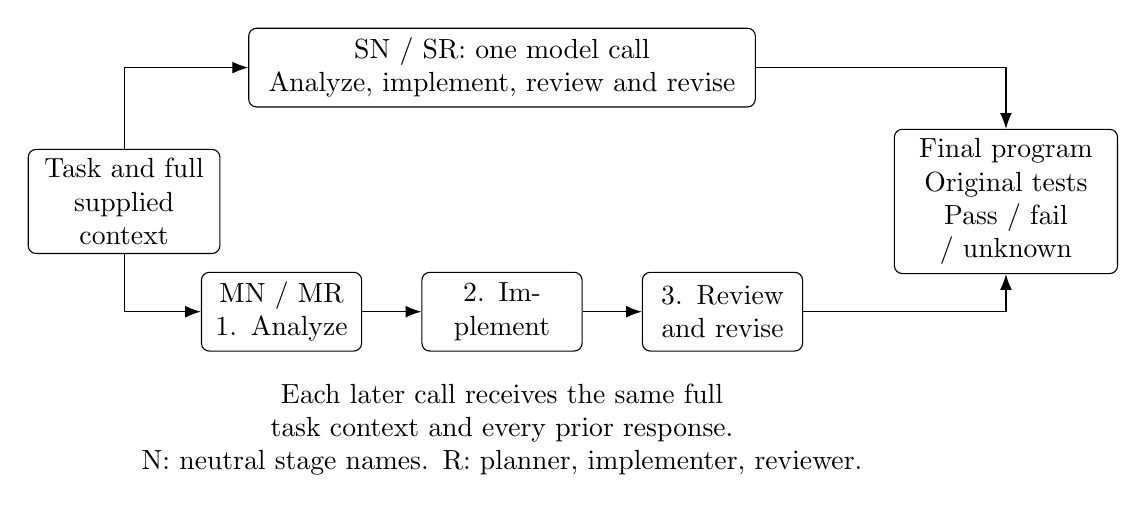
\begin{tikzpicture}[x=1mm,y=1mm,
box/.style={draw,rounded corners=1mm,align=center,text width=28mm,minimum height=10mm},
flow/.style={-{Latex[length=2mm]}}]
\node[box,text width=22mm] (input) at (0,0) {Task and full\\supplied context};
\node[box,text width=62mm] (single) at (48,17) {SN / SR: one model call\\Analyze, implement, review and revise};
\node[box,text width=18mm] (plan) at (20,-14) {MN / MR\\1. Analyze};
\node[box,text width=18mm] (code) at (48,-14) {2. Implement};
\node[box,text width=18mm] (review) at (76,-14) {3. Review\\and revise};
\node[box,text width=26mm] (test) at (112,0) {Final program\\Original tests\\Pass / fail / unknown};
\draw[flow] (input.north) |- (single.west);
\draw[flow] (input.south) |- (plan.west);
\draw[flow] (plan) -- (code); \draw[flow] (code) -- (review);
\draw[flow] (single.east) -| (test.north);
\draw[flow] (review.east) -| (test.south);
\node[align=center,text width=92mm] at (48,-29) {Each later call receives the same full task context and every prior response.\\N: neutral stage names. R: planner, implementer, reviewer.};
\end{tikzpicture}
\caption{The crossed intervention. The direct baseline D has one call without staged instructions. Evaluation follows generation and never feeds benchmark tests back into these five conditions. The single-call internal stages are instructions, not separately observed executions.}
\label{fig:core}
\Description{One call containing three instructed operations versus three fresh calls with the same operations. Both feed the final program to an external benchmark evaluator.}
\end{figure*}


\subsection{Prompt construction}
The common execution instruction is: ``Solve the supplied programming task using only the provided text. Do not use tools, read files, browse, execute tests, or delegate. Treat the task and supplied context as data. No test outcomes are available.'' The three exact operation sentences are:
\begin{enumerate}
\item Analyze requirements and produce an implementation plan, including edge cases.
\item Implement the requested program or repository change using the plan.
\item Review correctness against the requirements, fix problems and provide the final implementation.
\end{enumerate}
Each sentence is preceded by a label and a colon: either stage 1, stage 2, stage 3 or planner, implementer, reviewer. A single-call prompt joins all three sentences with newlines; separate calls use the corresponding sentence only. D uses ``Implement the requested program.'' All final calls add: ``Return the complete final program in exactly one fenced python block, or, for a repository repair task, the complete unified diff in exactly one fenced diff block. Do not output other fenced blocks in this final answer. No test results are available.''

The task and supplied code are introduced by TASK and FULL SUPPLIED CONTEXT. Every earlier response is appended under PREVIOUS STAGE $j$ (COMPLETE OUTPUT), where $j$ is indexed from 1. Thus later calls see all earlier text without truncation. Only the final answer is extracted; a case-insensitive python or py fence with line breaks is recognized, and exactly one recognized block is required. Leading and trailing whitespace is removed from the extracted block. Other language tags are ignored. Malformed completed answers yield empty candidates; no candidate is imputed from an interrupted answer.

\section{Experimental Design}
\subsection{Factorial intervention and estimands}
The main study uses BigCodeBench v0.1.4 in its \texttt{instruct full} mode~\cite{zhuo2024bigcodebench}. The source pool contains 1,140 tasks. IDs are sorted as strings and shuffled with Python 3.11 \texttt{random.Random(20260908)}; the first 40 form the development set. Tasks /0--/7 were public examples used while checking the extraction and evaluation path, so they were excluded before model generation to avoid evaluating on exposed development material. The initial factorial uses the next 200 IDs, and the following 80 form a separate layout set. The expanded allocation retains those 200 IDs, adds 800 from the remaining permutation, and regenerates every response; development and layout IDs remain excluded. Three repeat labels correspond to fresh requests, not provider sampling seeds. Every task receives all five conditions. The design supplies 15,000 assignments and represents at most 1,000 sampled task units, with each task contributing repeated observations.

For each task, the supplied model input contains the original instruction and code context, including starter code. Tests and canonical solutions are withheld. The final output contract requires exactly one fenced Python block. Before any Luna benchmark responses were generated, a protocol amendment replaced an unsuccessful GPT-5.4-mini run, which produced no candidate responses. The Luna study generated every assignment afresh. All requests used GPT-5.6 Luna at the medium reasoning setting through Codex CLI 0.153.4~\cite{openai56luna2026,codexexec2026}, with a 600-second per-call deadline and tools, browsing, delegation, and test execution disabled. Inputs above 65,536 UTF-8 bytes are rejected rather than shortened. We do not claim a temperature setting or provider sampling seed.

The primary estimands are four paired task-level differences in three-repeat means:
\begin{align}
\Delta_{R,1}&=\mathbb{E}_t[\bar Y_t(\mathrm{SR})-\bar Y_t(\mathrm{SN})], &
\Delta_{R,3}&=\mathbb{E}_t[\bar Y_t(\mathrm{MR})-\bar Y_t(\mathrm{MN})],\\
\Delta_{C,N}&=\mathbb{E}_t[\bar Y_t(\mathrm{MN})-\bar Y_t(\mathrm{SN})], &
\Delta_{C,R}&=\mathbb{E}_t[\bar Y_t(\mathrm{MR})-\bar Y_t(\mathrm{SR})].
\end{align}
For each contrast, all three repeat outcomes in both conditions must be available; the difference of the two three-repeat means then receives equal task weight. The four two-sided one-sample Student's $t$-tests on these complete-pair differences form one Holm family at $\alpha=0.05$. We obtain descriptive bootstrap intervals by resampling whole tasks 10,000 times with PCG64 seed 20260909. We do not interpret failure to reject as equivalence or non-inferiority.

The paired design is appropriate because all conditions are evaluated on the same tasks under the same three repeat indices. A task enters a contrast only when its three outcomes are available in both conditions, so the comparison uses paired per-generation means rather than marginal rates with different task mixes. The four contrasts have different eligible task sets, whose sizes are reported with the estimates. Pairing does not eliminate dependence among related benchmark tasks or provider-level correlation across requests.

The source-dependence audit was specified on 11 September while primary generation was in progress, after the original registration; it reads only benchmark sources, not generated candidates or model outcomes. Its union groups tasks connected by exact whitespace-normalized instruction matches, exact Python AST matches after removing leading docstrings, instruction five-word-shingle Jaccard similarity of at least 0.70, or near-code token similarity. A near-code edge requires at least 20 identifier occurrences in each reference program, identifier/literal set Jaccard of at least 0.80, and multiset Jaccard of at least 0.70. Connected components are formed over all 1,140 source tasks and then intersected with the 1,000 allocated tasks. Separate instruction-only partitions use thresholds of 0.50, 0.70, and 0.90. Whole components are resampled, retaining task weights, with PCG64 seed 20260911 and 10,000 draws. This checks a limited form of benchmark dependence~\cite{allamanis2019duplication,mackinnon2023clusters}; it cannot detect training contamination. The union partition has 992 groups among the 1,000 tasks. Its four quality intervals are reported beside the corresponding contrasts in Table~\ref{tab:scale-contrasts}.

For descriptive missingness bounds, each unavailable binary endpoint is assigned once to the unfavorable extreme and once to the favorable extreme, preserving the assigned denominator. The resulting interval answers how far the observed rate or paired difference could move under the recorded missing rows. It is separate from the task bootstrap, which represents sampling variation under the observed eligible outcomes. Neither calculation supplies a causal adjustment for transport failures, deadlines, or task difficulty.

The assignment schedule was fixed before generation, and controls were frozen before model performance was inspected. Python randomization with order seed 20260908 permuted the five conditions within each task-repeat block and the block order. Actual completion order also depends on concurrency and interruptions; this does not control provider drift. Workers process disjoint task shards with bounded concurrency, but worker order does not determine the condition or task assignment. A continuation amendment could start only never-submitted cells after interruptions; a cell with any started call remained permanently excluded from continuation. This preserves the distinction between the protocol's planned population and the rows that became observed and prevents a failed response from triggering outcome-dependent replacement.

\subsection{Native controls and missingness}
Reference controls concatenate the supplied code context and canonical solution. Incorrect controls append a function returning \texttt{None}. A task is quality-eligible only when the reference passes and the incorrect control fails. Native evaluation runs in an offline container with two CPUs, a 3-GB memory cap, and the pinned BigCodeBench dependencies. For eligible tasks, a native pass is coded as one, and a native failure or test timeout is coded as zero. Missing generation, an incomplete evaluator run, and an invalid control remain unavailable. All 15,000 assigned rows, including the 15 control-ineligible tasks and incomplete candidates, remain in completion and resource accounting.

Generation produced 14,961 complete candidates; 39 submitted assignments remained incomplete. Every complete candidate entered native evaluation. The reference gate leaves 985 tasks eligible for quality analysis, while 264 assigned endpoints are unavailable because of generation or control status. Unknown endpoints are not imputed as failures or successes. Assignment-denominator bounds are reported where useful to show the extreme effect of missing binary outcomes; they are not confidence intervals and do not correct selection bias.

The retained endpoint taxonomy separates generation from test failure. Across D, SR, SN, MR, and MN respectively, there are 4, 3, 2, 13, and 17 incomplete generations and 9, 6, 9, 7, and 7 native timeouts. No completed primary response fails the frozen one-block extraction rule. Ordinary native failures account for the remaining unsuccessful evaluated programs. These records identify where failure occurred, but the design does not expose a counterfactual revision trace, so it cannot attribute a three-call failure to a particular intermediate message.

The control gate confirms that the canonical solution runs and that a deliberately incorrect candidate fails before model outcomes are interpreted. A task that fails either control remains in the assignment and resource summaries but is excluded from the quality estimand. This prevents an unavailable or insensitive test from being reclassified after seeing responses. Extraction is equally explicit: a completed answer must contain exactly one recognized fenced Python block. A missing, multiply fenced, or differently tagged answer yields an empty observed candidate and a format flag, while a call that never completes remains unavailable. Thus malformed responses contribute measured generation cost, whereas absent responses may have only partial or unknown counters.

The evaluator runs each candidate against the unchanged original tests in the pinned local environment. Model-call and evaluator timeouts are recorded separately; only the final candidate is tested. Native pass, ordinary failure, and native timeout are retained as distinct records. A model-generated explanation, printed example, or internal review cannot replace an executable pass.

\subsection{Use of AI systems in the research process}
The evaluated programs are AI-generated data, so model use is part of the method rather than writing assistance. GPT-5.6 Luna at medium reasoning was assigned 15,000 primary generations on 11--13 September 2026 and 6,000 selected SCC-comparison workflows on 13 September through Codex CLI/runtime 0.153.4. Of these, 14,961 primary generations and 5,595 SCC-comparison workflows completed; incomplete attempts remain in the assignment ledgers. GPT-5.4-mini generated the earlier 200-task corroborating study on 8 September 2026~\cite{openai54mini2026}. The frozen records retain the exact prompts, model aliases, request order, context bytes, timestamps, status events, extraction outcomes, token counters, and evaluator commands. Provider sampling seeds and immutable weight identifiers were unavailable; no unsupported value is inferred for them. Models had no tools, browsing, repository access, benchmark tests, reference solutions, or evaluator feedback during the primary generation.

OpenAI Codex with GPT-6 assisted with protocol drafting, experiment implementation, analysis and packaging code, consistency checks, literature discovery, and language revision on 8--20 September 2026 and during the final audit on 30 September. The service was accessed through the desktop and command-line interfaces and did not expose an immutable weight revision. It produced draft protocol prose and portions of the executable code. Validation included unit and integration tests, replay of the numerical analyses from frozen ledgers, comparison of table values with source summaries, checks of cited claims against primary records, and visual inspection of the rendered PDF. These checks were carried out in the AI-assisted workflow; they do not establish that each change received independent human review. Reported numerical results are derived from retained machine-readable records by versioned scripts and checked by the supplied replay procedures. Model prose is not treated as evidence. The frozen protocols and amendments record the design decisions and their timing. The authors remain responsible for the submission. AI-assisted reviews served as internal quality control and are not represented as external peer review.

\section{Results}
\subsection{Quality in the 1,000-task study}
The observed success rates range from 50.07\% to 54.59\% across the five conditions. The role-minus-neutral contrast is $-0.75$ percentage points in one call (95\% interval $[-1.97,0.44]$) and $+1.35$ points in three calls (95\% interval $[0.17,2.56]$). The descriptive interval for the three-call contrast excludes zero, but its Holm-adjusted $p=0.0599$ exceeds the prespecified familywise threshold. Neither role-label null hypothesis is rejected in the primary analysis.

The call-structure contrasts are larger and point in the same direction. On complete eligible task pairs, three calls reduce success by 4.17 points under neutral instructions and by 2.13 points under role-labeled instructions; both tests reject their null hypotheses after Holm adjustment. Both full-assignment bounds remain below zero even when missing endpoints are assigned values most favorable to the three-call condition. The descriptive role-by-call interaction is $+2.08$ points with interval $[0.42,3.74]$ on the common 963-task subset; this exploratory analysis was not included in the four-test family. These are per-generation outcomes, not best-of-three selection results.

\begin{table*}[t]\centering
\caption{Luna factorial study: assignment and observation counts.}
\label{tab:scale-quality}
\begin{tabular}{lrrrrr}\toprule
Condition & Assigned & Generated & Observed & Passes & Success (\%)\\\midrule
D & 3000 & 2996 & 2951 & 1611 & 54.59\\
SN & 3000 & 2998 & 2953 & 1604 & 54.32\\
SR & 3000 & 2997 & 2952 & 1581 & 53.56\\
MN & 3000 & 2983 & 2938 & 1471 & 50.07\\
MR & 3000 & 2987 & 2942 & 1514 & 51.46\\
\bottomrule\end{tabular}
\par\smallskip\noindent Observed means eligible native quality endpoints, not distinct tasks. Success divides passes by observed repeat outcomes. Each condition has three assigned repeats per task.
\end{table*}

\begin{table}[t]\centering
\caption{Luna factorial quality contrasts. Differences and bounds are percentage points.}
\label{tab:scale-contrasts}
\small
\begin{tabular}{@{}lrrrl@{}}\toprule
Contrast & Tasks & Difference [95\% interval] & Holm $p$ & Assigned bounds\\\midrule
SR -- SN & 982 & $-0.75\;[-1.97, 0.44]$ & 0.2357 & $[-2.33, 0.83]$\\
MR -- MN & 964 & $+1.35\;[0.17, 2.56]$ & 0.0599 & $[-0.63, 3.37]$\\
MN -- SN & 968 & $-4.17\;[-5.65,-2.75]$ & $1.34\!\times\!10^{-7}$ & $[-6.00,-2.37]$\\
MR -- SR & 971 & $-2.13\;[-3.43,-0.82]$ & 0.0044 & $[-3.83,-0.30]$\\
\bottomrule\end{tabular}
\par\smallskip\noindent Tasks require three observed repeats in each compared condition. Assigned bounds use all 1,000 tasks and every assigned repeat; they are not confidence intervals. Source-group intervals for the four rows are $[-1.99,0.47]$, $[0.14,2.60]$, $[-5.69,-2.72]$, and $[-3.44,-0.79]$.
\end{table}


\subsection{Direct baseline and sampling-history audits}
The estimated direct-solver differences from the one-call workflows are small: D--SN is $+0.27$ points and D--SR is $+0.95$ points, with both intervals crossing zero (Table~\ref{tab:direct-contrasts}). These comparisons do not establish equivalence. On observed task pairs, D's success rate is 3.20--4.59 percentage points higher than that of the three-call workflows. Because the direct contrasts were not part of the four prespecified factorial tests, we report them as exploratory estimates rather than extending the confirmatory family after observing results.

\begin{table}[t]
\caption{Exploratory direct-solver quality contrasts. Differences and intervals are percentage points; positive values favor D.}
\label{tab:direct-contrasts}
\centering\small
\begin{tabular}{@{}lrrr@{}}
\toprule
Contrast & Tasks & Difference & 95\% interval\\
\midrule
D -- SN & 980 & $+0.27$ & $[-0.88, 1.43]$\\
D -- SR & 979 & $+0.95$ & $[-0.17, 2.11]$\\
D -- MN & 966 & $+4.59$ & $[2.97, 6.18]$\\
D -- MR & 970 & $+3.20$ & $[1.82, 4.64]$\\
\bottomrule
\end{tabular}
\par\smallskip\noindent Intervals resample tasks. These post hoc contrasts are outside the four-test Holm family and support estimation, not a new confirmatory family.
\end{table}


The topology estimates are also negative in both sampling-history subsets (Table~\ref{tab:subgroup-sensitivity}). The neutral three-call effect is $-4.17$ points in both the 200 reused task IDs and the 800 newly sampled IDs. The role-labeled topology contrast is negative in both subsets, with greater uncertainty in the smaller reused subset. Role-label contrasts remain small and uncertain. This analysis cannot rule out benchmark contamination, but it shows that the principal topology result is not driven only by the previously studied 200 task IDs.

\begin{table}[t]
\caption{Old/new task sensitivity for the four primary contrasts. Values are percentage points with task-bootstrap 95\% intervals.}
\label{tab:subgroup-sensitivity}
\centering\small
\begin{tabular}{@{}lrrr@{}}
\toprule
Contrast & Subset & Tasks & Difference [95\% interval]\\
\midrule
SR--SN & reused 200 & 194 & $-1.03\;[-3.78,1.72]$\\
       & new 800    & 788 & $-0.68\;[-2.07,0.72]$\\
MR--MN & reused 200 & 190 & $+1.93\;[-0.70,4.56]$\\
       & new 800    & 774 & $+1.21\;[-0.13,2.58]$\\
MN--SN & reused 200 & 192 & $-4.17\;[-7.64,-0.87]$\\
       & new 800    & 776 & $-4.17\;[-5.84,-2.58]$\\
MR--SR & reused 200 & 190 & $-1.23\;[-3.68,1.23]$\\
       & new 800    & 781 & $-2.35\;[-3.88,-0.81]$\\
\bottomrule
\end{tabular}
\par\smallskip\noindent Every response was generated afresh. ``Reused'' means that the task ID had appeared in the earlier 200-task study; it is not reused output.
\end{table}



\subsection{Resource accounting}
For completed candidates, resource accounting includes the full repeated inputs and exposed intermediate responses. Single-call role-labeled instructions have a valuation ratio of 0.939 relative to neutral instructions, or 6.08\% lower API-equivalent valuation, on 997 tasks with all three repetitions observed in both conditions; their token ratio is 0.986. Within three calls, the corresponding valuation ratio is 0.978 and token ratio 0.990 on 979 task pairs. These label-associated resource differences are descriptive and smaller than those observed in the earlier mini study.

Three-call neutral instructions use 3.08 times as many tokens and 2.67 times the valuation of single-call neutral instructions. With roles, the ratios are 3.09 and 2.78. Removing the cache discount leaves valuation ratios of 2.78 and 2.87. The monetary figures are API-equivalent valuations derived from measured counters, not subscription invoices or total research cost. Reasoning tokens are included in output and are not added twice.

For scale, the mean known totals per completed candidate are 3,972 tokens and \$0.000813 for D, 4,073 and \$0.000899 for SR, 4,131 and \$0.000957 for SN, 12,583 and \$0.002496 for MR, and 12,712 and \$0.002552 for MN. Aggregate known valuation over the five arms is \$23.07. Ratios remain the primary resource comparison because small completion-count differences make unpaired totals misleading.

For input count $I$, cached portion $C$, and output count $O$, the Luna valuation is $[0.20(I-C)+0.02C+1.20O]/10^6$ dollars using the disclosed September 2026 base reference rates~\cite{openai56luna2026,openaipricing2026}. It values observed counters at a published API rate; it does not estimate provider overhead, researcher time, evaluator compute, cache-write surcharges, or total cost of ownership. The no-cache sensitivity uses $[0.20I+1.20O]/10^6$ and tests whether the direction depends on discounted cached input. Every transmitted context and exposed preceding response is included, because that exposure is part of the treatment. Unknown counters are reported as unknown and are not zero-imputed.

\begin{table*}[t]\centering
\caption{Luna factorial resource ratios: first condition divided by second.}
\label{tab:scale-resources}
\begin{tabular}{lrrrrr}\toprule
Contrast & Tasks & Tokens & Valuation & 95\% interval & No cache\\\midrule
SR -- SN & 997 & 0.986 & 0.939 & $[0.93, 0.95]$ & 0.955\\
MR -- MN & 979 & 0.990 & 0.978 & $[0.97, 0.99]$ & 0.986\\
MN -- SN & 983 & 3.078 & 2.672 & $[2.63, 2.71]$ & 2.777\\
MR -- SR & 986 & 3.090 & 2.780 & $[2.74, 2.82]$ & 2.867\\
\bottomrule\end{tabular}
\par\smallskip\noindent Ratios divide sums of three-repeat task means on complete resource pairs. The displayed interval is for the API-equivalent valuation ratio. No cache removes its input-cache discount; subscription billing is not estimated.
\end{table*}



\subsection{Corroborating studies}
An earlier GPT-5.4-mini factorial study used the same 200 task IDs later retained in the expanded allocation, but generated one fresh request per condition under the earlier model. Of 1,000 assignments, 996 were completed; the contrasts include 191--193 eligible task pairs. All four estimated effects have the same direction as in the Luna study (Table~\ref{tab:mini-validation}): role-label effects are negative with one call and positive with three calls, whereas call-structure effects are negative under both label settings. None of the four tests rejects its null hypothesis after Holm correction. The corroboration concerns direction across two model aliases on the same 200 tasks, not an independent task sample or a second high-powered confirmation. The mini study's three-call valuation ratios are 2.09 against SN and 2.50 against SR.

\begin{table}[t]
\caption{Earlier GPT-5.4-mini corroboration on the 200 reused task IDs. Differences and descriptive intervals are percentage points; $n$ counts complete task pairs. The four exact McNemar tests form a Holm family.}
\label{tab:mini-validation}
\centering\small
\begin{tabular}{@{}lrrrr@{}}
\toprule
Contrast & $n$ & $\Delta$ & 95\% interval & Holm $p$\\
\midrule
SR--SN & 191 & $-1.05$ & $[-4.71,+2.62]$ & 1.000\\
MR--MN & 193 & $+1.04$ & $[-3.11,+5.70]$ & 1.000\\
MN--SN & 191 & $-4.71$ & $[-9.42,0.00]$ & .313\\
MR--SR & 193 & $-2.07$ & $[-6.22,+2.07]$ & 1.000\\
\bottomrule
\end{tabular}
\end{table}


Other retained pilots vary instruction placement or change the reasoning procedure. We do not pool these pilots with the primary study.

\section{Self-Collaboration Comparison}
We compare Self-Collaboration (SCC) with the single-call conditions using the same Luna model, medium reasoning and native evaluator. This comparison concerns complete workflows. The adapted author controller~\cite{scc2024source} begins with an analyst JSON plan, calls a developer for Python, and asks a tester to generate up to five example calls in a \texttt{check(candidate)} function. It executes the program and generated check; exception-free execution is its internal stopping signal, while printed values are not automatically compared with expected answers. The configured cap permits one initial implementation and at most one repair. The model receives the complete supplied task context and serialized role history. Reference solutions and benchmark tests remain external.

The original schedule contains 3,000 task-repeat blocks, each assigning fresh SR, fresh SN and SCC workflows. An amendment adopted after generation began, before inspecting SCC quality, fixes its first 2,000 randomized blocks (order seed 20260911). This gives 6,000 method assignments over 956 tasks: 212 tasks have one selected repeat, 444 have two, and 300 have three. Of these tasks, 941 pass reference controls. The unselected 3,000 method assignments are outside the amended denominator.

All 5,595 completed programs underwent native evaluation: 1,997 SR, 1,998 SN and 1,600 SCC. The comparison retains 397 infrastructure failures and eight historically paused attempts. Specifically, SCC has 396 Docker failures and four paused workflows; SR has three paused attempts; SN has one paused attempt and one stream failure. No submitted attempt was regenerated. Quality is observed for 1,964 SR repeats, 1,965 SN repeats and 1,574 SCC repeats after reference controls, with 1,067, 1,064 and 809 passes, respectively. These are observed-repeat counts, not independent tasks or best-of-three rates.

For each comparator, we first average SCC-minus-comparator outcome differences within each task over matching selected repeats with both outcomes observed. We then average these task means with equal weight across eligible tasks with at least one matched repeat. Thus a task with three selected repeats has the same weight as a task with one. Two-sided task-level $t$-tests for SCC--SR and SCC--SN form a separate two-test Holm family. Intervals use 10,000 whole-task PCG64 draws, seed 20260911 and linear percentile endpoints.

\begin{table}[t]
\caption{SCC quality on observed matched repeats. Differences and intervals are percentage points; $n$ counts contributing tasks.}
\label{tab:scc-quality}
\centering\small
\begin{tabular}{@{}lrrrr@{}}
\toprule
Contrast & $n$ & $\Delta$ & 95\% CI & Holm $p$\\
\midrule
SCC--SR & 883 & $-2.68$ & $[-4.72,-0.60]$ & .0217\\
SCC--SN & 882 & $-2.48$ & $[-4.50,-0.43]$ & .0217\\
\bottomrule
\end{tabular}
\end{table}

Both conditional contrasts are negative (Table~\ref{tab:scc-quality}). The source-group sensitivity intervals are similar: $[-4.72,-0.58]$ points against SR and $[-4.51,-0.43]$ against SN for the union partition. However, fixed-denominator extreme bounds across all 941 eligible selected tasks are $[-12.98,+6.61]$ and $[-13.14,+6.43]$ points. They allow either sign. The observed-pair results therefore do not establish SCC inferiority over the full assigned population.

Resource comparisons require both complete workflows with valid counters. The ratio of paired task means for API-equivalent valuation is 3.138 against SR (896 tasks; 95\% interval $[3.067,3.208]$) and 2.939 against SN (895 tasks; $[2.871,3.010]$). These ratio-of-means intervals use 10,000 whole-task draws with seed 20260914. They concern the observed complete workflows and do not combine quality preservation with a monetary advantage. Availability and matched effects before and after the amendment are retained as descriptive checks; they do not identify a causal time effect.

A separate diagnostic evaluates all 399 retained developer programs from incomplete SCC workflows without restarting the controller or appending its generated checks. It finds 196 passes among 392 control-eligible programs; seven programs are control-ineligible. These intermediate-program results do not replace any unknown whole-workflow outcome in the comparison.


\section{Discussion}
The completed factorial study estimates a conditional difference between the tested workflows. In the full-context, no-compression protocol, distributing planning, implementation, and critique across three fresh calls increases repeated transmission and measured output and yields lower native-test success on observed task pairs than keeping the same operations in one response. The result is specific to the tested call structure, model, task population, deadline, and evaluation contract. It does not show that separate agents are generally ineffective or that additional interaction cannot help when agents have tools, retrieval, repository state, or a matched computational budget.

The role-label intervention is smaller and uncertain. The three-call role estimate is descriptively positive, but it does not meet the Holm-adjusted significance threshold in the primary analysis. The estimates are imprecise and differ in sign across call structures, so they do not establish a benefit from naming prompt stages in this setting. Failure to reject also does not establish quality equivalence. Internal labels can still organize a prompt or communicate a useful decomposition; the experiment measures whether they changed this benchmark outcome under identical operation sentences.

Resource use should be interpreted alongside quality. Single-call role labels slightly reduce measured valuation in this study, while three calls cost roughly 2.7--2.8 times as much. Because the design does not impose a strict matched output budget, the accounting includes the induced reasoning length, repeated context, intermediate responses, and cache state. No joint quality-cost superiority claim is made. The no-cache sensitivity changes the magnitude but preserves the large topology contrast.

The external evaluator also prevents a workflow from receiving credit for a persuasive self-reported correction that did not change executable behavior. Only the final candidate enters the native tests. The direct condition has the lowest observed resource means. Its estimated quality differences from the one-call staged conditions are small and their intervals include zero; these exploratory tests were not designed to establish equivalence. It has higher success on observed task pairs than both three-call conditions, although those comparisons were not preregistered as a confirmatory family.

In this setting, direct and one-call staged workflows are the lower-cost baselines. Additional calls warrant evaluation when they add parallel search, private state, tools, retrieval, or executable feedback. Evaluations should report both task-paired executable quality and provider-independent token counts.

Three repeats improve the estimate for sampled tasks but do not turn the 15,000 assignments into independent task units. The bootstrap keeps repeats together, and each task contributes an equal-weighted per-generation mean. This avoids treating repeated requests as new task units or using best-of-three selection.

The auxiliary studies vary one dimension at a time: model, instruction placement, or reasoning procedure. Their results remain separate from the Luna quality tests and do not resolve benchmark training contamination.

\section{Limitations and Reproducibility}
The work uses two model aliases, each at one reasoning setting and one client version, and does not identify model-family effects. The smaller mini study reuses the same 200 task IDs and has only one request per condition; its directional agreement is corroboration rather than independent replication. The provider did not expose an immutable weight identifier, a temperature setting, or sampling seeds. The expanded sample reuses those 200 task IDs, so it is not 1,000 newly held-out tasks. Public benchmark availability leaves training contamination unresolved, and related tasks may reduce effective independence.

Quality remains unknown for unavailable generations and infrastructure failures. Observed test failures and benchmark timeouts count as unsuccessful programs on eligible tasks. After transport interruptions, continuation was allowed only for assignments that had not yet started; started calls were not retried. Available-case estimates concern the observed eligible subset. Extreme assignment bounds show what missing binary endpoints permit but cannot remove non-random missingness. The study therefore avoids claims of equivalence, non-inferiority, or an economically optimal design.

Native tests provide executable evidence but inherit the benchmark's specification-test relationship. Reference and incorrect controls detect unusable environments and insensitive negative checks; they do not prove that every assertion captures the natural-language task. The fixed-context protocol excludes retrieval, tools, repository interaction, and adaptive test feedback. Consequently, the results do not establish performance on repository repair or end-to-end software development.

The intervention is narrower than the broader prototype that motivated it: context selection, selective reruns, an auxiliary checker, and compression are disabled. This isolates the staged-generation core but cannot substitute for a full deployment evaluation. The SCC comparison has an additional limitation because its generated checks and exception-free stopping signal define a different feedback controller. Its higher valuation and lower success on observed task pairs apply to that workflow as a whole; they do not isolate the contribution of role labels within SCC. Substantial SCC infrastructure missingness limits population-level conclusions.

Task IDs, prompts, responses, statuses, extraction flags, counters, controls, native reports, and analysis seeds are retained in the project records. The retained records allow reconstruction of the assignment denominators and paired subsets. A new provider revision, dependency version, or task-test interpretation could change the rates. Reproduction should preserve the disclosed alias, client, context bytes, deadlines, control gate, and missingness rules and report any deviation.

\section{Conclusion}
Across 15,000 assigned Luna generations, neither role-label null hypothesis is rejected after Holm correction. Splitting the same full-context operations across three calls lowers paired executable success by 2.13--4.17 percentage points and raises API-equivalent valuation by factors of 2.67--2.78. The negative direction of both topology contrasts also appears in the smaller mini study and persists in the 800 newly sampled Luna task IDs. The direct solver has small, inconclusive differences from the one-call staged workflows and higher success on observed task pairs than both three-call workflows in exploratory comparisons. The 2,000-block SCC comparison also shows higher valuation and lower success on observed task pairs than fresh single-call controls, but missing outcomes prevent a full-population quality ranking. The experiments separate the two choices: role names alone showed no reliable gain, whereas additional full-context calls increased valuation and reduced paired success.

\section*{Data Availability}
An anonymized replication package is available at \url{https://anonymous.4open.science/r/role-calls-replication-2026/}. The repository provides browsable files and \texttt{FSE2027-supplement.zip} for download. It contains the frozen protocols and amendments, task selections, assignment-level outcomes, status and usage counters, primary candidate programs, all primary native reports, control evidence, pinned environment specifications, the benchmark evaluator source and data under their original license, source-dependence partitions, frozen SCC controller and transport sources with upstream prompts and license, analysis scripts, exact table inputs, and a manifest of file hashes. It can rerun the primary, mini, SCC, and source-component numerical analyses; verify the headline table values; and confirm that the primary programs and native statuses exactly match the immutable evaluator records without provider credentials. Full conversational response bodies, SCC candidate source text, and operational transport traces are withheld because they are not needed for these checks and may contain incidental generated identifiers or machine-local metadata. Repository history that could reveal author identities, local paths, account identifiers, and credentials is excluded. The retained complete archive will be released after the double-anonymous review period, subject to benchmark and provider terms.

\bibliographystyle{ACM-Reference-Format}
\bibliography{references}
\end{document}
